\documentclass{article}
\usepackage[utf8]{inputenc}

\title{Intelligent Optimization of Machine Learning Methods\\[0.8em]Final Report}
\author{Jonathan Gillett}
\date{August 2015}

\usepackage{natbib}
\usepackage{graphicx}
\usepackage{url}
\usepackage{setspace}
\usepackage{floatrow}
\usepackage{xcolor}
\usepackage{amsmath}

\newcommand{\bold}[1]{\textbf{#1}}

\begin{document}

\maketitle


\section{Project Definition}

Machine Learning is a branch of Computer Science that has since evolved from the study of pattern recognition and computational theory into a highly diverse and widely used area of research. This evolution has empowered society with the almost limitless amount of data that has become available\cite{lohr2012age, mohri2012foundations}.

Machine Learning focuses on the creation of algorithms, often rooted in artificial intelligence methods; in order to learn from, model, and make predictions based on data rather than following deterministic program instructions\cite{dietterich2002machine, bishop2006pattern}. These algorithms frequently involve the analysis and understanding of large data sets, often referred to as ``Big Data'', which are seemingly insurmountable using traditional statistical methods\cite{lohr2012age}. However, with the use of Machine Learning methods, models are created based on the data, in order to make predictions or decisions, 

The increase in the sheer volume and the variety of data requires advances in methodology to automatically understand, process, and summarize data. As such, this has created a huge demand for Machine Learning techniques, which are applied to data for performing clustering analysis, dimensionality reduction, and modelling to better understand and predict trends. Clustering analysis involves algorithms for grouping or clustering objects according to measured or perceived intrinsic characteristics or similarity; making it possible to find patterns which would otherwise be indistinguishable\cite{jain2010}. 

Clustering is one of the most important methods in Machine Learning, with K-means being one of the most popular clustering algorithms. Given the widespread use and applications of K-means, the goal of the research has been to enhance the performance of K-means using the intelligent methods of Genetic Algorithms (GA) to reduce the requirement of domain knowledge. While many researchers have attempted to minimize the requirement of domain knowledge such as by selecting better initial centroid points\cite{meilua2006uniqueness}, limiting the need to specify the number of clusters\cite{tibshirani2001estimating}, or improving the similarity criteria\cite{kashima2008k}. There has been little work done in using Evolutionary Strategies such as GA, to optimize these parameters.

As such, the main focus of this research project has been to enhance the robustness and accuracy of the widely used K-means clustering method using Evolutionary Strategies such as GA to optimize the domain knowledge parameters, making it more robust to a wide variety of problems and further enhancing the accuracy and effectiveness.




\section{Project Importance}

Clustering, which is often referred to as cluster analysis, is an essential process in machine learning that focuses on discovering the natural groupings of a set of patterns, points, or objects within the data. Clustering is one of the most important methods in Machine Learning, with K-means being one of the most popular clustering algorithms. K-means remains the most popular method of clustering, it was independently discovered by Lloyd and MacQueen\cite{lloyd1982least, macqueen1967some} and has been widely used for over 50 years. The reason for K-means popularity is that it is one of the simplest clustering algorithms and still produces reasonable results for most applications.

However, despite it's widespread adoption, K-means is not without problems, K-means, and by extension nearly all clustering methods are very dependent on several factors which can require domain knowledge from an expert. In the case of K-means, in order to achieve optimal clustering the following parameters must be specified by an expert with domain knowledge: initial centroids, number of clusters, and similarity criteria. Furthermore, in particular for K-Means clustering, in order to find an optimal clustering, the operation is \bold{NP-Hard}\cite{jain2010}, making the problem computationally infeasible for highly dimensional or very large data sets, which is often the case when applying Machine Learning methods to Big Data.

Therefore, any improvements made to K-means would have a profound impact on the accuracy and effectiveness of the method. In addition, the enhancements from the research project, using Evolutionary Strategies such as GA, would make the methods more generalized and able to adapt to the diversity of data from different problem domains without requiring domain knowledge.




\section{K--means}

K-means is the most widely used clustering method and is essential to discovering the natural groupings of a set of patterns, points, or objects within the data. Formally, all clustering methods can be described as follows:\\

\emph{Given a representation of $N$ objects, find $K$ groups based on a measure of similarity such that the similarities between objects in the same group are high while the similarities between objects in different groups are low}\cite{jain2010}.\\

Based on this definition, and as a result of the similarity criteria for clustering, it can be expected that clustering is a subjective entity that often is in the eye of the beholder and whose significance and interpretation requires domain knowledge from an expert. As a result of the requirement for domain knowledge, this has resulted in thousands of clustering algorithms being published for use, and that continue to appear\cite{jain2010}, further emphasizing the need for an intelligent clustering method that evolves to the problem space.

K-means has a rich and diverse history as it was independently discovered in multiple scientific fields prior to it's formalization and independent publication by Lloyd (published in 1982)\cite{lloyd1982least} and MacQueen (published in 1967)\cite{macqueen1967some}. Despite the fact that K-means was first proposed over 50 years ago, it is still one of the most widely used algorithms for clustering\cite{jain2010}.

The K-means algorithm is powerful in it's simplicity, from a high-level perspective the algorithm can be described as the following:


\begin{enumerate}
\item The data is clustered by first determining a set of centroid points

\item The algorithm then finds a partition, such that the squared error between the empirical mean of a cluster and the centroid points in the cluster is minimized\cite{macqueen1967some, lloyd1982least}.

\end{enumerate}


As outlined independently by MacQueen and Lloyd in their publications of the K-means clustering algorithm, it can be formally described in mathematical terms as follows.\\

Let $X = {x_i}, i = 1, \ldots, n$ be the set of $n$ $d$-dimensional points to be clustered into a set of $K$ clusters, $C = {c_k, k = 1, \ldots, K}$. K-means algorithm finds a partition such that the squared error between the empirical mean of a cluster and the points in the cluster is minimized. Let $\mu_k$ be the mean of the cluster $c_k$, the squared error between $\mu_k$ and $c_k$ is defined as follows.

\begin{equation}
J(c_k) = \sum_{x_i \in c_k}^{} \|x_i - \mu_x\|^{2}
\label{eq:kmeans1}
\end{equation}

Where the optimization criteria of K-means is to minimize the sum of the squared error over all K clusters.

\begin{equation}
J(C) = \sum_{k = 1}^{K} \sum_{x_i \in c_k}^{} \|x_i - \mu_x\|^{2}
\label{eq:kmeans2}
\end{equation}


The main reasons for the continued popularity of K-means is due to the ease of implementation, simplicity, and efficiency\cite{jain2010}. The subsequent 50 years of development in clustering algorithms have been based on the equations \ref{eq:kmeans1} and \ref{eq:kmeans2} for K-means. 

While K-means has been the most popular clustering algorithm, the original algorithm does not take into consideration any information about the problem domain; limiting it's accuracy and robustness. It is for this very reason that the focus of this research project is to optimize the parameters of K-means using GA, without the requirement of an expert's domain knowledge.

Lastly, it is important to note that the K-means optimization criteria for the final clustering, as described in equation \ref{eq:kmeans2}, which minimizes the sum of the squared error over all $K$ clusters is \bold{NP-HARD}\cite{drineas2004clustering}.




\section{Genetic Algorithms}

Evolutionary Strategies, in particular Genetic Algorithms (GA) are the core aspect of the enhancement to K-means, GA are used to optimize the parameters of K-means, which often requires an expert's domain knowledge, without any knowledge from an expert.

GA by their definition are inspired by nature, similar to nature, GA use the concept of evolution in order to ``evolve'' a solution to a problem over the course of many generations. GA are artificial evolution; a population evolves under rules which determine the fitness of the strongest individuals in the population, which pass on their genes to future generations\cite{golberg1989genetic, haupt2004practical}.

Given the unique approach to optimization and problem solving that GA have they as such are non-linear in nature, and are often able to solve highly complex and dynamical systems\cite{negnevitsky2011artificial}. As such, GA are very commonly used in optimization, however there are many other applications that they can have, for the purpose of the research project GA were ideal in order to optimize the clustering parameters without requiring domain knowledge.

The earliest origins of GA are rooted in Charles Darwin’s theory of evolution presented before the Linnean Society of London. The methodology of GA was first developed by John Holland in 1975, and popularized by David Goldberg in 1989, who demonstrably used GA to optimize gas-pipeline transmission\cite{golberg1989genetic}.

Modern biological evolutionary theory is based on the processes of reproduction, mutation, competition, and selection. GA attempts to mimic the process of evolution artificially by describing or encoding a problem as a chromosome, performing reproduction selectively based on the fitness of chromosomes to simulate ``survival of the fittest'', and lastly the breeding and mutation of offspring\cite{golberg1989genetic, negnevitsky2011artificial}.

The entire GA process can be described as follows based on the following ten step process and proceeding flowchart described by Negnevitsky\cite{negnevitsky2011artificial}.


\begin{enumerate}

\item Represent the problem as a chromosome of a fixed length, choose the size of the chromosome population $N$, the crossover probability $P_c$ and the mutation probability $P_m$.

\item Define a fitness function, $f(x)$, to measure the performance of each chromosome. The fitness function determines the likelihood that chromosomes will be mated during reproduction (survival of the fittest).

\item Generate a random initial population $x_1 \ldots x_N$ of chromosomes of size $N$.

\item Calculate the fitness $f(x_i)$ of each individual chromosome in the population.

\item Select a pair of chromosomes for mating from the current population. The chromosomes are selected with a probability $p_i$ related to their fitness, such that the higher fitness (stronger) chromosomes have a higher probability of being selected for mating than less fit chromosomes (survival of fittest).

\item Create a pair of offspring chromosomes by applying the genetic operators of crossover and mutation.

\item Place the created offspring chromosomes in the new population.

\item Repeat \bold{step 5} (selecting chromosomes from the population) until the size of the new chromosome population becomes equal to the size of the initial population, $N$.

\item Replace the initial (parent) chromosome population with the new (offspring) population.

\item Go to \bold{step 4}, and repeat the process until the termination criterion is satisfied.

\end{enumerate}


% GA FLOWCHART
\begin{figure}[H]
\centering
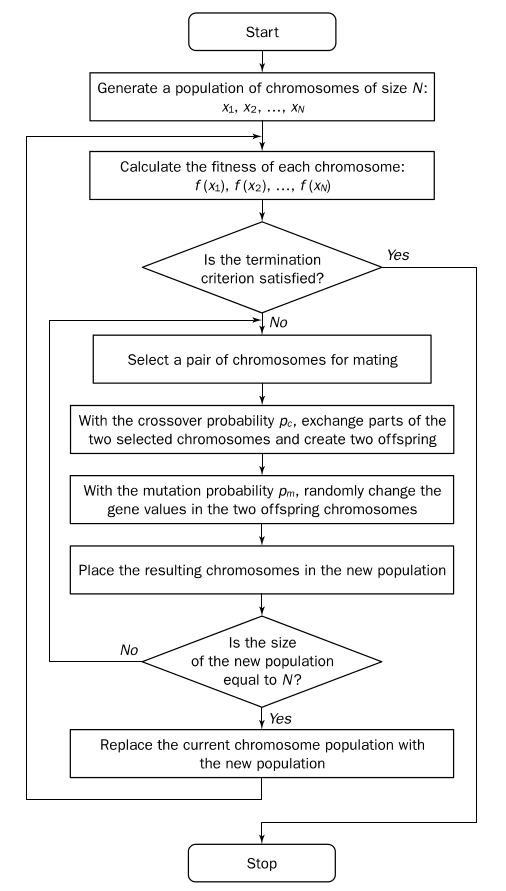
\includegraphics[width=0.85\textwidth]{figures/ga-flowchart}
\caption{Genetic Algorithm Flowchart\cite{negnevitsky2011artificial}}.
\label{fig:ga-flowchart}
\end{figure}




\section{Evolutionary K--means (E--means) Algorithm}

The course project solution is the \emph{Evolutionary} K-means (\emph{E-means}) algorithm, which is an enhancement to the K-means algorithm by using the powerful optimization and problem solving capabilities of GA to optimize the clustering parameters rather than requiring an expert's domain knowledge. With nearly all clustering algorithms, and by extension K-means, the following parameters must be specified by an expert with domain knowledge: initial centroids, number of clusters, and similarity criteria.

For the purpose of the initial \emph{E-means} research project implementation, only the most challenging parameter, the selection of centroids, was optimized using GA. Ideally, it would be the most beneficial to have all three parameters optimized using GA and not require any domain knowledge, however this has proven to be difficult and computationally intensive as each parameter must be a separate independent GA process, with each of the independent GA optimizations for each parameter dependent on the outcome of the previous. Thus, in order to limit the number of variables being tested for the purpose of the research project to \emph{one}, only the selection of the centroid points is optimized using GA.

The \emph{E-means} operation depends on the following GA configurations in order to optimize for the centroids: a chromosome structure, a fitness functions, and the genetic operators crossover and mutation.


\subsection{Chromosome Structure}

In order to encode the centroids of each cluster in the form of a chromosome, each centroid is represented as a vector, the centroids for each cluster are then stored as a row in a matrix, where each row of the matrix is a cluster, and the columns are the values of the centroid vector for that cluster.

The following is the matrix representation of a chromosome in the population for the iris flower data set\cite{bezdek1999will} used for the research project.

\begin{equation}
A = \begin{bmatrix}
    5.374303   & 2.108351   & 4.088924   & 1.993956 \\
    5.282249   & 3.500251   & 5.993241   & 1.208288 \\
    5.773559   & 2.218215   & 2.471298   & 1.644890 
\end{bmatrix}
\label{eq:chromosome}
\end{equation}


\subsection{Fitness Function}

In order to evaluate the fitness of the chromosomes in the population, and how good the final clustering is as a result of the centroid points, the Dunn Index was used. The Dunn Index is an internal evaluation scheme, meaning it evaluates based on the current clustering results how well the values are clustered, where a higher Dunn index indicates better clustering\cite{dunn1973fuzzy}. Thus, a chromosome with centroids that results in a clustering with a higher Dunn Index, provides a more superior clustering result, and thus higher fitness, increasing it's chance of passing it's solution onto the next generation.


\subsection{Genetic Operators}

The genetic operators, crossover and mutation, are performed on the chromosomes, which contain the centroids for each cluster represented as matrices, as shown in equation \ref{eq:chromosome}.

For the mutation operation, the operator randomly selects a row, $r_i$ (cluster), and column, $c_j$, in the chromosome matrix, and changes the value to a random value within the acceptable bounds $[min(c_j), max(c_j))$ for that column.

The following is a demonstration of mutation using the chromosome shown in equation \ref{eq:chromosome}, where $r_i = 2$ and  $c_j = 3$ and the result of the mutation operation is $A^{\prime}$.


\begin{align*}
A &= \begin{bmatrix}
    5.374303   & 2.108351   & 4.088924   & 1.993956 \\
    5.282249   & 3.500251   & \color{red}5.993241   & 1.208288 \\
    5.773559   & 2.218215   & 2.471298   & 1.644890 
    \end{bmatrix}\\
A^{\prime} &= \begin{bmatrix}
    5.374303   & 2.108351   & 4.088924   & 1.993956 \\
    5.282249   & 3.500251   & \color{red}2.115234   & 1.208288 \\
    5.773559   & 2.218215   & 2.471298   & 1.644890 
    \end{bmatrix}
\label{eq:mutation}
\end{align*}


For the crossover operation, the the operator randomly selects a row, $r_i$,  as the crossover point, and randomly selects a side, $s$ as either ``left'' or ``right'' of the crossover point. It then swaps the values before, or after the crossover point based on the side, between parent $A$ and parent $B$.

The following is a demonstration of the crossover operation using two parents, chromosomes $A$ and $B$, where the crossover point is $r_i = 2$ and $s = left$, and the resultant offspring of the crossover operation are $A^{\prime}$ and $B^{\prime}$.

\begin{align*}
A &= \textcolor{red}{\begin{bmatrix}
    5.374303   & 2.108351   & 4.088924   & 1.993956 \\
    5.282249   & 3.500251   & 5.993241   & 1.208288 \\
    5.773559   & 2.218215   & 2.471298   & 1.644890 
    \end{bmatrix}}\\
B &= \textcolor{blue}{\begin{bmatrix}
    4.348525   & 3.546295   & 1.953808   & 0.113626 \\
    6.805044   & 3.144741   & 4.517384   & 1.369251 \\
    6.584664   & 3.305431   & 1.195916   & 1.953624
    \end{bmatrix}}\\
A^{\prime} &= \begin{bmatrix}
    \color{blue}4.348525   & \color{blue}3.546295   & \color{blue}1.953808   & \color{blue}0.113626 \\
    \color{blue}6.805044   & \color{blue}3.144741   & \color{blue}4.517384   & \color{blue}1.369251 \\
    \color{red}5.773559   & \color{red}2.218215   & \color{red}2.471298   & \color{red}1.644890 
    \end{bmatrix}\\
B^{\prime} &= \begin{bmatrix}
    \color{red}5.374303   & \color{red}2.108351   & \color{red}4.088924   & \color{red}1.993956 \\
    \color{red}5.282249   & \color{red}3.500251   & \color{red}5.993241   & \color{red}1.208288 \\
    \color{blue}6.584664   & \color{blue}3.305431   & \color{blue}1.195916   & \color{blue}1.953624
    \end{bmatrix}
\end{align*}


\section{Implementation}

In terms of the implementation, much care was taken to ensure that the code would have the best performance possible, as optimization and Machine Learning methods are often computationally intensive. In addition, the main focus was to also ensure that the code would be compliant with the latest programming standards, and easily utilized by other researchers by ensuring there is detailed documentation.

The code was written purely in C to have the most optimal performance possible, the C99 standard\cite{c99} was used, so that code is compliant and up-to-date with modern programming standards.

In addition to being written in C99, the BLAS/LAPACK libraries were used for linear algebraic operations to provide an additional performance increase. These libraries are written in FORTRAN and provide the optimal performance for the low level operations performed using Lloyd's algorithm, which is used in the clustering process. As well, in order to simplify the development of the code and reduce the amount of non-essential code needed, the library Libconfuse was used to provide configuration file support.

In order to ensure there was an optimal uniformly random number generator (PRNG), the PCG algorithm library was used, which provides excellent randomness with low periodicity, which is ideal for performing GA operations.

It was initially intended to use MPI for massive parallelization, but this proved to be very challenging given the complex data structure of the chromosomes and cluster solutions, which are multi-dimensional matrices.

The code was designed to be very adaptable, other researchers and academics interested in utilizing the code simply have to modify or create a configuration file to use the E-means algorithm. This makes it easy for other researchers and academics to evaluate the viability of E-means by testing it with their existing problems and data sets, they can then compare results and draw their own conclusions with ease.

Lastly, all of the code is Open Source, licensed under the GNU General Public License (GPL) to make it as accessible as possible for everyone.




\section{Methodology}

\begin{enumerate}

\item Establish a set of test data that is widely used for benchmarking and comparing clustering and dimensionality reduction algorithms in the Machine Learning community.

\item Implement the standard algorithms for clustering, K-means.

\item Execute the standard K-means algorithm with each of the test data sets in order to establish a basis to compare to the enhanced implementations.

\item Implement the enhanced K-means clustering algorithms using a single or combination of multiple intelligent methods (e.g. Evolutionary Computation).

\item Execute the clustering algorithms enhanced using intelligent methods with the test data in order to evaluate the solutions.

\item Compare the results of the enhanced algorithms to the standard algorithms, focusing on improvements in the accuracy and adaptability of the enhanced solution to different problem domains and the performance improvements of parallelization.

\end{enumerate}






\section{Results}

The results of the E-means algorithm were calculated using the iris flower data set,\footnote{While the iris data set was first published in the 1930's, the corrected version by Bezdek was used for the purpose of the research project.} which is a very common data set used in Machine Learning when demonstrating classification and clustering algorithms\cite{bezdek1999will}. Specifically, the iris flower data set was chosen because the amount of data is reasonable in size and therefore easily comprehensible, as well it has also been used numerous times in literature when demonstrating clustering algorithms\cite{ben2002support, jiang2001two, horn2001algorithm}.

At first the initial iris flower data set was used, however after thorough literature review we discovered that the original data set published by Fisher in 1936, \emph{The Use of Multiple Measurements in Taxonomic Problems}\cite{fisher1936use}, contains numerical errors. Thus we chose to use the corrected version of the original data set published by Bezdek in \emph{Will the Real Iris Data Please Stand Up?}\cite{bezdek1999will}.

For the purpose of the test, the standard K-means algorithm, using Lloyd's algorithm, with 10 trials was executed using the specified number of clusters, $K = 3$, and Euclidean length as the similarity criteria. For each trial the fitness of the clustering solution was calculated using the Dunn Index, the results of the trials using the standard K-means algorithm can be seen in the figure \ref{fig:kmeans-performance}.

% KMEANS PERFORMANCE
\begin{figure}[H]
\centering
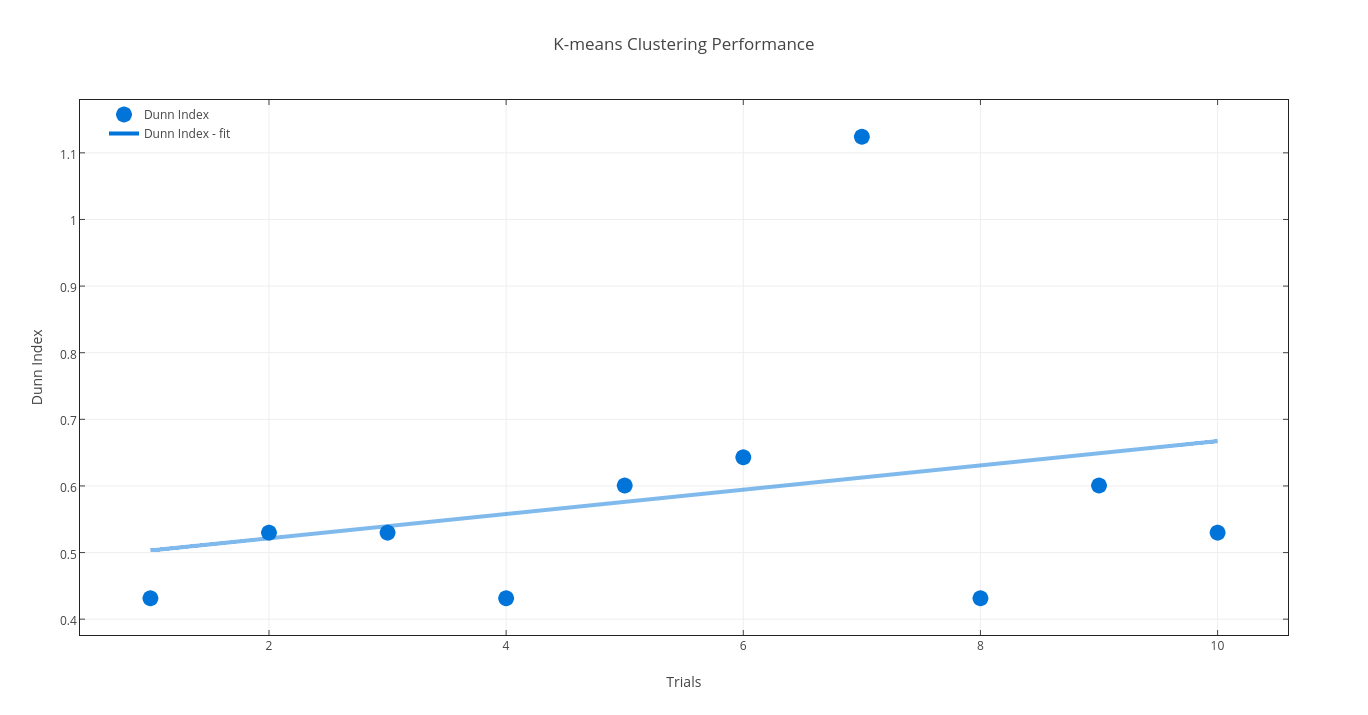
\includegraphics[width=\textwidth]{figures/kmeans-performance}
\caption{Performance of K-means algorithm measured using the Dunn Index for 10 trials.}
\label{fig:kmeans-performance}
\end{figure}

The E-means algorithm was executed with the same parameters as K-means, $K = 3$ and the Euclidean length as similarity criteria as well as similar cluster performance and time constraints. The GA was configured to optimize the centroids using a population of 10 chromosomes, with a total of 10 generations. The E-means algorithm was tested against the exact same iris data set as the standard K-means algorithm implementation. The fitness of the E-means solutions were calculated using the Dunn Index, the results of which can be seen in figure \ref{fig:emeans-performance}.

% EMEANS PERFORMANCE
\begin{figure}[H]
\centering
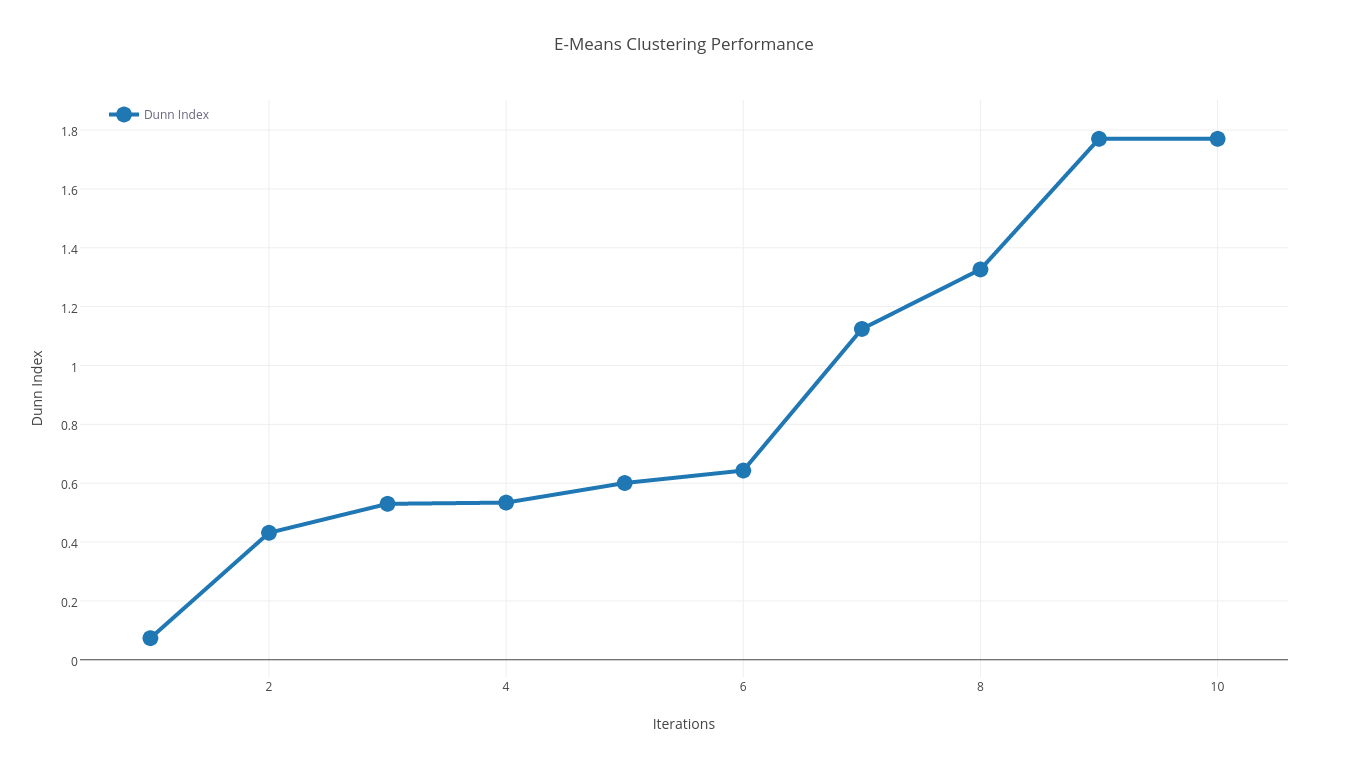
\includegraphics[width=\textwidth]{figures/emeans-performance}
\caption{Performance of E-means algorithm measured using the Dunn Index for 10 generations.}
\label{fig:emeans-performance}
\end{figure}


Comparing the results between figure \ref{fig:kmeans-performance} for the K-means algorithm and figure \ref{fig:emeans-performance} for the E-means algorithm the differences between the two solutions becomes evident. In figure \ref{fig:kmeans-performance} we see the sporadic approach to finding the optimal clustering using multiple trials, while in one trial, based on the Dunn Index, a near optimal clustering solution was found, the approach does not have the ability to intelligently search for the optimal centroids for clustering. In contrast, as shown in figure \ref{fig:emeans-performance} the E-means algorithm quickly approaches the optimal solution of a Dunn Index of \bold{1.770231} within only 10 generations.

Furthermore, it is worthwhile to mention that throughout our tests we were never able to find any clustering solution with a Dunn Index greater than 1.770231, even after executing the E-means solution for \bold{100,000} generations.



\section{Conclusions}

Clustering is a quintessential component of Machine Learning, with K-means being one of the most popular clustering algorithms. In our research project we set out to enhance the the performance of K-means using the intelligent methods of Genetic Algorithms (GA) to reduce the requirement of domain knowledge, which can be hard to determine, especially when working with Big Data.

We proposed a novel new algorithm, based on the foundations of the most widely used clustering algorithm, K-means, enhancing it using Genetic Algorithms (GA) to optimize the centroids parameter, rather than requiring they be specified using domain knowledge. We named our new algorithm, \emph{Evolutionary} K-means (\emph{E-means}) emphasizing that it is an enhancement to the K-means algorithm using the powerful optimization and problem solving capabilities of GA. By utilizing the optimization capabilities of GA, the centroids are able to be chosen optimally without requiring domain knowledge by an expert, freeing them to focus on remaining two parameters: the number of clusters desired and the similarity criteria for comparing data points.

Our solution provides a unique approach to performing K-means clustering more optimally, reducing the need for researchers to perform computationally expensive calculations in order to determine the optimal clustering for K-means, which is NP-HARD\cite{jain2010}. As demonstrated in the \emph{Results} section, the E-means algorithm, optimizes for the centroids parameter, which is critical for an optimal clustering, and evaluates the fitness of the resultant clustering using the Dunn Index\cite{dunn1973fuzzy}, which is widely used for evaluating the results of clustering algorithms.

The results from our research shown in figures \ref{fig:kmeans-performance} for K-means and figure \ref{fig:emeans-performance} for E-means, show the distinct difference between the two approaches. For the K-means results we see a sporadic approach to finding the optimal clustering using multiple trials, while in the E-means results we see it clearly approaching the optimal solution by optimizing the centroids using GA, rather than a Monte-Carlo random trials approach used by the K-means algorithm.

In conclusion, we set out to enhance the robustness and accuracy of the widely used K-means clustering method using the Evolutionary Strategies of GA to optimize the domain knowledge parameters. We chose to focus on optimizing the most difficult parameter, the centroids, and our results supported the improvements from GA when applied to the K-means algorithm for selecting the optimal centroids.


\bibliographystyle{plain}
\bibliography{references}
\end{document}
